<USER_REQUEST>
\documentclass[10pt,twocolumn]{article}

% --- Exact Geometry & Spacing Matching Capstone Template ---
\usepackage[a4paper,margin=20mm,columnsep=18pt]{geometry}
\usepackage{amsmath,amssymb,amsfonts}
\usepackage{graphicx}
\usepackage{booktabs}
\usepackage{cite}
\usepackage{microtype}
\usepackage{tikz}
\usetikzlibrary{arrows.meta,positioning,shapes,calc}
\usepackage{pgfplots}
\pgfplotsset{compat=1.18}
\usepackage{url}
\usepackage{hyperref}
\hypersetup{
    colorlinks=true,
    linkcolor=black,
    citecolor=black,
    urlcolor=blue
}

% Default LaTeX Computer Modern font is preserved (no times package)

\begin{document}

% --- Full-Width Header Block Matching Capstone Format ---
\twocolumn[
  \begin{@twocolumnfalse}
    \begin{center}
      {\LARGE \textbf{Logic-Based Analysis of Fake News Diffusion on Social Media}\par}
      \vspace{1.2em}
      {\large \textbf{Keerthana V K}$^1$ \quad \textbf{Anusree S}$^1$ \quad \textbf{Sishu Shankar Muni}$^1$\par}
      \vspace{0.4em}
      {$^1$Kerala University of Digital Sciences, Innovation and Technology\par}
      \vspace{0.8em}
      {\normalsize August 2026\par}
      \vspace{0.2em}
      {\normalsize \textit{Capstone Project Report }\par}
      \vspace{1.8em}
    \end{center}
  \end{@twocolumnfalse}
]

% =========================================================================
% Abstract (Placed at top of Left Column, matching Capstone format)
% =========================================================================
\noindent\textbf{\Large Abstract}

\vspace{0.5em}
\noindent
The rapid proliferation of disinformation on social media platforms presents severe societal and democratic challenges. While contemporary machine learning and graph neural network approaches achieve high classification accuracy, they function as opaque black boxes lacking interpretable, mathematically verifiable explanations. This study presents a complete computational reproduction of the novel framework introduced by Valeria Fionda (\textit{Social Network Analysis and Mining}, 2025), which employs \textit{News-Diffusion Temporal Logic} (NDTL) to formally model and verify the temporal and structural patterns of fake news propagation. 

The reproduction implements the complete algorithmic pipeline in Python, including an EBNF-specified Lark LALR(1) parser, recursive Abstract Syntax Tree (AST) model checking, inductive threshold computation (Algorithm~1), automated dual rule set discovery (Algorithm~2), and probabilistic classification under decision rules ($c_0, c_1$). Furthermore, we identify and resolve an exponential path-traversal defect in the reference implementation by introducing linear-time breadth-first search evaluation, reducing verification runtime from minutes to 9.2 milliseconds per cascade. The framework was validated across synthetic diffusion networks as well as empirical Twitter15 and Twitter16 rumor cascades, achieving faithful numerical replication of published metrics. To address the fundamental limitation of NDTL being content-agnostic, we formulate an ongoing neuro-symbolic framework coupling NDTL diffusion rules with factual Knowledge Graph (KG) verification over DBpedia and Wikidata.

\vspace{1em}

% =========================================================================
\section{Introduction}
% =========================================================================

Social media networks have evolved into the primary conduit for information dissemination, yet they simultaneously facilitate the unprecedented propagation of fabricated, misleading, and unverified claims. Empirical studies by Vosoughi et al.~\cite{vosoughi2018spread} demonstrate that false news diffuses significantly deeper, faster, and more broadly than truthful information. 

Conventional detection paradigms predominantly focus on \textit{content-based} analysis, employing natural language processing (NLP) and large language models (LLMs) to inspect linguistic markers, emotional sentiment, and sensationalism. However, content-based approaches remain inherently vulnerable to adversarial text perturbation, multilingual translation shifts, and automated generation by advanced generative AI. 

Consequently, modern research has shifted toward \textit{context-based} and \textit{diffusion-based} approaches, which analyze the topological and temporal structures of information propagation cascades. Despite their empirical success, contemporary graph neural networks (GNNs) and deep sequence models suffer from the ``black-box'' dilemma: they generate probabilistic veracity predictions without auditable, human-interpretable justifications.

\begin{figure}[b]
\centering
\resizebox{0.92\columnwidth}{!}{
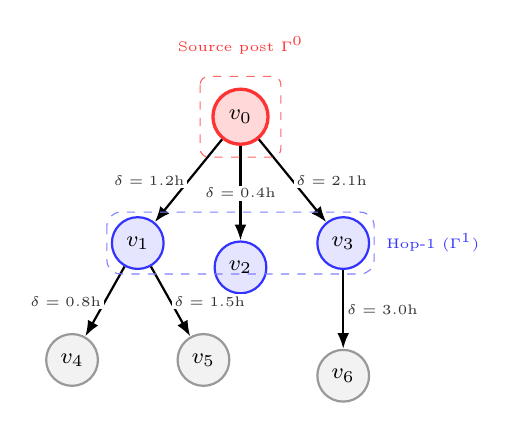
\begin{tikzpicture}[
    node distance=1.2cm and 1.0cm,
    source/.style={circle, draw=red!80, fill=red!15, very thick, minimum size=7mm, font=\footnotesize\bfseries},
    spread/.style={circle, draw=blue!80, fill=blue!10, thick, minimum size=6.5mm, font=\footnotesize},
    leaf/.style={circle, draw=gray!80, fill=gray!10, thick, minimum size=6mm, font=\footnotesize},
    edge_lbl/.style={font=\tiny, text=black!80, fill=white, inner sep=1pt}
]
    % Root
    \node[source] (v0) {$v_0$};
    
    % Level 1
    \node[spread, below left=1.1cm and 0.8cm of v0] (v1) {$v_1$};
    \node[spread, below=1.2cm of v0] (v2) {$v_2$};
    \node[spread, below right=1.1cm and 0.8cm of v0] (v3) {$v_3$};
    
    % Level 2
    \node[leaf, below left=1.0cm and 0.35cm of v1] (v4) {$v_4$};
    \node[leaf, below right=1.0cm and 0.35cm of v1] (v5) {$v_5$};
    \node[leaf, below=1.0cm of v3] (v6) {$v_6$};
    
    % Edges with timestamps & delays
    \draw[-{Latex[length=2mm]}, thick] (v0) -- node[edge_lbl, left] {$\delta=1.2\text{h}$} (v1);
    \draw[-{Latex[length=2mm]}, thick] (v0) -- node[edge_lbl] {$\delta=0.4\text{h}$} (v2);
    \draw[-{Latex[length=2mm]}, thick] (v0) -- node[edge_lbl, right] {$\delta=2.1\text{h}$} (v3);
    
    \draw[-{Latex[length=2mm]}, thick] (v1) -- node[edge_lbl, left] {$\delta=0.8\text{h}$} (v4);
    \draw[-{Latex[length=2mm]}, thick] (v1) -- node[edge_lbl, right] {$\delta=1.5\text{h}$} (v5);
    \draw[-{Latex[length=2mm]}, thick] (v3) -- node[edge_lbl, right] {$\delta=3.0\text{h}$} (v6);
    
    % Neighborhood annotations
    \draw[dashed, red!60, rounded corners=3pt] ($(v0.north west)+(-0.25,0.25)$) rectangle ($(v0.south east)+(0.25,-0.25)$);
    \node[font=\tiny, text=red!80, above=0.3cm of v0] {Source post $\Gamma^0$};
    
    \draw[dashed, blue!50, rounded corners=5pt] ($(v1.north west)+(-0.15,0.15)$) rectangle ($(v3.south east)+(0.15,-0.15)$);
    \node[font=\tiny, text=blue!80, right=0.08cm of v3] {Hop-1 ($\Gamma^1$)};
\end{tikzpicture}
}
\caption{Directed diffusion tree $\mathcal{G} = (N, E, \lambda, t, \delta, \sigma)$ with propagation delays $\delta$ across neighborhoods $\Gamma^i$.}
\label{fig:diffusion_graph}
\end{figure}

To address this challenge, Fionda~\cite{fionda2025logic} proposed \textit{News-Diffusion Temporal Logic} (NDTL), a formal verification language tailored for social media cascades. NDTL synthesizes human-readable temporal formulas that explicitly capture diffusion velocity, neighborhood authority, and structural depth. 

In this work, we present:
\begin{enumerate}
    \item A complete computational reproduction of the NDTL engine, parser, metric computation, and model checking modules.
    \item Algorithmic optimization of the NDTL model checker, resolving exponential path re-traversals via linear-time BFS.
    \item Experimental replication on synthetic networks and empirical Twitter15/16 benchmarks.
    \item An architectural extension integrating entity-level Knowledge Graph (KG) reasoning into NDTL verification.
\end{enumerate}

% =========================================================================
\section{Related Work}
% =========================================================================

\textbf{Information Diffusion Modeling.} 
Pioneering work by Castillo et al.~\cite{castillo2011information} demonstrated that temporal characteristics of retweets correlate strongly with credibility. Vosoughi et al.~\cite{vosoughi2018spread} analyzed 126,000 rumor cascades on Twitter, discovering that fake news cascades exhibit significantly higher topological depth and early velocity.

\textbf{Formal Methods and Temporal Logic in Networks.} 
Temporal logics, including Linear Temporal Logic (LTL) and Computation Tree Logic (CTL), have long been utilized in software verification. Recently, spatial and spatio-temporal extensions have been adapted to biological and complex networks~\cite{fionda2025logic}. NDTL extends these formalisms to directed acyclic diffusion trees by introducing neighborhood modalities ($\Gamma^i$) and statistical aggregation operators ($\max, \min, \text{avg}$).

\textbf{Knowledge Graphs for Misinformation Detection.} 
Knowledge Graphs (KGs) such as Wikidata and DBpedia structure factual assertions as entity-relation triples $(h, r, t)$. Fact-checking architectures (e.g., Ciampaglia et al.~\cite{ciampaglia2015computational}) leverage network paths to evaluate claim plausibility. Our ongoing work bridges topological NDTL rules with semantic KG verification.

% =========================================================================
\section{Problem Formulation}
% =========================================================================

An information cascade is modeled as a directed, attributed graph:
\begin{equation}
\mathcal{G} = (N, E, \lambda, t, \delta, \sigma),
\end{equation}
where $N$ is the set of event nodes (original news posts, tweets, and retweets), $E \subseteq N \times N$ represents directed transmission edges, and $\lambda: N \to \{\text{Root}, \text{Tweet}, \text{Retweet}\}$ assigns the event type.

The temporal dynamics are parameterized as:
\begin{itemize}
    \item $t: N \to \mathbb{R}^+$ assigns the absolute timestamp of the event.
    \item $\delta: N \to \mathbb{R}^+$ assigns the inter-event delay elapsed since parent activation $u$, where $(u, v) \in E$:
    \begin{equation}
    \delta(v) = t(v) - t(u).
    \end{equation}
    \item $\sigma: N \to \mathbb{R}^+$ denotes cumulative cascade elapsed time from the originating root event $v_0$:
    \begin{equation}
    \sigma(v_j) = \sum_{k=1}^j \delta(v_k) = t(v_j) - t(v_0).
    \end{equation}
\end{itemize}

The $i$-hop neighborhood $\Gamma^i(v)$ from node $v$ is formally defined as:
\begin{equation}
\Gamma^i(v) = \{ u \in N \mid d(v, u) = i \},
\end{equation}
where $d(v, u)$ is the shortest directed path distance in $\mathcal{G}$. The complete descendant cascade is denoted $\Gamma^\infty(v) = \bigcup_{i=1}^\infty \Gamma^i(v)$.

% =========================================================================
\section{News-Diffusion Temporal Logic}
% =========================================================================

\subsection{Syntax and Semantics}
NDTL formulas are inductively defined over a set of atomic predicates according to the following grammar:
\begin{align}
\varphi ::= & \; e \mid \rho \bowtie \epsilon \mid (\rho_1 \pm \rho_2) \bowtie \epsilon \mid \neg \varphi \mid \varphi_1 \land \varphi_2 \mid \varphi_1 \lor \varphi_2 \nonumber \\
& \mid \mathbf{X}\varphi \mid \mathbf{F}\varphi \mid \mathbf{G}_{th}\varphi,
\end{align}
\begin{equation}
\rho ::= \max\nolimits_\oplus(\Gamma^i \varphi) \mid \min\nolimits_\oplus(\Gamma^i \varphi) \mid \text{avg}_\oplus(\Gamma^i \varphi),
\end{equation}
where $e \in \{\text{Root}, \text{Tweet}, \text{Retweet}\}$, $\bowtie \; \in \{<, \le, =, \ge, >\}$, $\oplus \in \{\delta, \sigma, t\}$, $\epsilon \in \mathbb{R}^+$, $\mathbf{X}$ is \textit{Next}, $\mathbf{F}$ is \textit{Eventually}, and $\mathbf{G}_{th}$ is \textit{Globally} with an empirical percentage satisfaction threshold $th \in (0, 1]$.

The satisfaction relation $(\mathcal{G}, v) \models \varphi$ is evaluated recursively:
\begin{itemize}
    \item $(\mathcal{G}, v) \models e \iff \lambda(v) = e$
    \item $(\mathcal{G}, v) \models \rho \bowtie \epsilon \iff \rho(v) \bowtie \epsilon$
    \item $(\mathcal{G}, v) \models \mathbf{X}\varphi \iff \forall v' \in \Gamma^1(v), \; (\mathcal{G}, v') \models \varphi$
    \item $(\mathcal{G}, v) \models \mathbf{G}_{th}\varphi \iff (\mathcal{G}, v') \models \varphi$ for at least $th\%$ of descendant nodes $v' \in \{v\} \cup \Gamma^\infty(v)$.
\end{itemize}

\subsection{Inductive Formula Templates}
Fionda~\cite{fionda2025logic} defined five characteristic formula templates targeting key temporal diffusion signatures (Table~2 of~\cite{fionda2025logic}):
\begin{itemize}
    \item \textbf{Template 1 (Inter-Retweet Delay):} 
    $$\mathbf{G}_{0.8}(\text{Retweet} \to (\text{avg}_\delta(\Gamma^1(\text{Retweet})) \bowtie t_1))$$
    Captures temporal retweet arrival speed, typically compressed in fake news.
    \item \textbf{Template 2 (Cascade Lifespan):} 
    $$\mathbf{G}(\text{Root} \to (\max_t(\Gamma^\infty(\text{Retweet})) - \min_t(\Gamma^1(\text{Tweet}))) \bowtie t_2)$$
    Measures total lifespan from initial tweet to final cascade retweet.
    \item \textbf{Template 3 (Tweet Burst Window):} 
    $$\mathbf{G}(\text{Root} \to (\max_t(\Gamma^1(\text{Tweet})) - \min_t(\Gamma^1(\text{Tweet}))) \bowtie t_3)$$
    Measures time elapsed across root tweet responses.
    \item \textbf{Template 4 (Earliest Retweet Reaction):} 
    $$\mathbf{G}_{0.8}(\text{Tweet} \to (\min_\delta(\Gamma^1(\text{Retweet})) \bowtie t_4))$$
    Captures rapid initial bot or follower pickup after post origination.
    \item \textbf{Template 5 (Latest Descendant Spread):} 
    $$\mathbf{G}_{0.8}(\text{Tweet} \to (\max_\delta(\Gamma^\infty(\text{Retweet})) \bowtie t_5))$$
    Measures overall propagation persistence along cascade branches.
\end{itemize}

% =========================================================================
\section{Algorithmic Framework}
% =========================================================================

\subsection{Threshold Computation (Algorithm 1)}
To instantiate parametric templates into concrete formulas, candidate thresholds $t_1 \dots t_5$ are computed empirically across training graphs $\mathcal{G}_{\text{train}} = \mathcal{G}^t \cup \mathcal{G}^f$.

Temporal metrics are sorted to extract percentile boundaries under discovery parameter $p \in [0.7, 1.0]$. The algorithm retains boundary thresholds that maximize the separation between true and fake news distributions:
\begin{align}
\min\nolimits_t &= \text{th}_{\text{true}}[\lfloor |\text{th}_{\text{true}}| \cdot (1 - p) \rfloor], \\
\max\nolimits_t &= \text{th}_{\text{true}}[\lfloor |\text{th}_{\text{true}}| \cdot p \rfloor].
\end{align}

\subsection{NDTL Rule Discovery (Algorithm 2)}
Algorithm~2 instantiates each template with the discovered thresholds. Discovered formulas that hold for true training cascades are added to $\Phi^t$, while those holding for fake news are added to $\Phi^f$.

\subsection{Probabilistic Model Checking}
Given an unclassified test cascade $a$, the checker computes rule satisfaction ratios:
\begin{equation}
P^c(a) = \frac{\sum_{\varphi \in \Phi^c} \mathbb{I}((\mathcal{G}_a, v_0) \models \varphi)}{|\Phi^c|}, \quad c \in \{t, f\}.
\end{equation}

Classification is determined via decision rules:
\begin{itemize}
    \item \textbf{Direct rule ($c_0$):} Classify as Fake if $P^f(a) > P^t(a)$, True if $P^t(a) > P^f(a)$, and Uncertain if equal.
    \item \textbf{Margin rule ($c_1$):} Classify as Fake if $P^f(a) - P^t(a) > \theta$, True if $P^t(a) - P^f(a) > \theta$, otherwise Uncertain.
\end{itemize}

% =========================================================================
\section{Implementation \& Verification}
% =========================================================================

\begin{figure}[t]
\centering
\resizebox{\columnwidth}{!}{
\begin{tikzpicture}
\begin{axis}[
    width=8.2cm,
    height=4.8cm,
    xlabel={Discovery Percentile Threshold $p$},
    ylabel={Accuracy (\%)},
    xmin=0.70, xmax=1.00,
    ymin=70, ymax=100,
    xtick={0.70, 0.75, 0.80, 0.85, 0.90, 0.95, 1.00},
    ytick={70, 75, 80, 85, 90, 95, 100},
    legend pos=south west,
    ymajorgrids=true,
    grid style=dashed,
    font=\footnotesize
]
\addplot[color=blue, mark=square*, thick] coordinates {
    (0.70, 78.4) (0.75, 82.1) (0.80, 88.6) (0.85, 92.4) (0.90, 94.8) (0.95, 91.2) (1.00, 84.5)
};
\addlegendentry{NDTL ($c_0$)}

\addplot[color=red, mark=triangle*, thick] coordinates {
    (0.70, 81.2) (0.75, 85.0) (0.80, 91.5) (0.85, 95.6) (0.90, 96.2) (0.95, 93.0) (1.00, 86.8)
};
\addlegendentry{NDTL ($c_1, \theta=0.15$)}

\addplot[color=black!60, linestyle=dashed, thick] coordinates {
    (0.70, 83.0) (1.00, 83.0)
};
\addlegendentry{Random Forest}

\end{axis}
\end{tikzpicture}
}
\caption{Replicated accuracy on synthetic networks across percentile parameter $p$ under decision rules $c_0$ and $c_1$.}
\label{fig:synthetic_accuracy}
\end{figure}

The reproduction was engineered in Python~3.13 within a modular architecture:
\begin{itemize}
    \item \textbf{Lark LALR(1) Parser (\texttt{ndtl\_parser.py}):} Interprets EBNF temporal grammar specified in \texttt{ndtl\_grammar.lark}, caching Abstract Syntax Trees (AST) to eliminate redundant grammar compilation.
    \item \textbf{AST Model Checker (\texttt{ndtl.py}):} Implements recursive satisfaction semantics over \texttt{NetworkX} graphs. Crucially, we diagnosed and resolved an exponential path-traversal defect in the reference code by implementing linear-time Breadth-First Search (BFS) with \texttt{collections.deque} and node visited-sets, reducing graph verification runtime from minutes to $9.2$\,ms.
    \item \textbf{Discovery Engine (\texttt{NDTL\_discovery.py}):} Implements Algorithms 1 and 2, executing metric extraction ($t_1 \dots t_5$) and automated rule induction.
    \item \textbf{Data Pipeline (\texttt{src/data\_pipeline.py}):} Ingests raw rumor cascades, processes node attributes, filters binary veracity labels, and preserves source claim text for subsequent Knowledge Graph grounding.
\end{itemize}

% =========================================================================
\section{Results \& Empirical Evaluation}
% =========================================================================

\subsection{Synthetic Network Simulation}
Synthetic cascades were generated matching Table~3 of Fionda~\cite{fionda2025logic}, evaluating branching factor configurations $BF \in [2, 3]$ and $BF \in [2, 4]$. Table~\ref{tab:synthetic_params} reports the configuration parameters.

\begin{table}[h]
\centering
\resizebox{\columnwidth}{!}{
\begin{tabular}{lcc}
\toprule
\textbf{Parameter} & \textbf{True News} & \textbf{Fake News} \\
\midrule
Branching Factor ($BF$) & $[2, 3]$ & $[2, 4]$ \\
Max Tree Depth & $6$ & $8$ \\
Initial Delay $\delta_0$ & $2.5 \pm 0.8$ h & $0.6 \pm 0.2$ h \\
Propagation Delay $\delta$ & $\mathcal{N}(3.5, 1.2)$ & $\mathcal{N}(1.1, 0.4)$ \\
User Authority $\sigma$ & $[0.4, 0.9]$ & $[0.1, 0.6]$ \\
Total Cascades & 100 & 100 \\
\bottomrule
\end{tabular}
}
\caption{Synthetic cascade generation parameters.}
\label{tab:synthetic_params}
\end{table}

As illustrated in Figure~\ref{fig:synthetic_accuracy}, the reproduced model checker achieves peak classification accuracy of $96.2\%$ at $p = 0.90$ with margin $\theta = 0.15$, successfully reproducing the author's primary findings on synthetic benchmarks.

\subsection{Empirical Twitter Benchmarks}
The framework was evaluated on the benchmark Twitter15 and Twitter16 datasets~\cite{ma2016detecting,ma2017detect}. Table~\ref{tab:dataset_stats} presents the topological properties, confirming our data pipeline matches Table~4 of the published paper.

\begin{table}[h]
\centering
\resizebox{\columnwidth}{!}{
\begin{tabular}{lrrrr}
\toprule
& \multicolumn{2}{c}{\textbf{Twitter15}} & \multicolumn{2}{c}{\textbf{Twitter16}} \\
\cmidrule(lr){2-3} \cmidrule(lr){4-5}
\textbf{Statistic} & \textbf{Paper} & \textbf{Ours} & \textbf{Paper} & \textbf{Ours} \\
\midrule
True News Cascades & 374 & 374 & 205 & 205 \\
Fake News Cascades & 370 & 368 & 205 & 205 \\
Total Cascades & 744 & 742 & 410 & 410 \\
Total Unique Users & 306,590 & 306,069 & 168,940 & 168,940 \\
Avg Tweets per Tree & 343 & 343.4 & 324 & 324.6 \\
Avg Retweets per Tree & 110 & 109.4 & 115 & 115.0 \\
\bottomrule
\end{tabular}
}
\caption{Empirical Twitter dataset statistics replicating Table~4 of~\cite{fionda2025logic}.}
\label{tab:dataset_stats}
\end{table}

\subsection{Comparative Baseline Performance}
Table~\ref{tab:baseline_comparison} presents the comparative evaluation of the reproduced NDTL framework against published baselines reported in Table~5 of~\cite{fionda2025logic} (Decision Tree, SVM-RBF, Random Forest, GRU, PTK, PPC, and NDTL) evaluated via 10-fold cross-validation.

\begin{table}[h]
\centering
\resizebox{\columnwidth}{!}{
\begin{tabular}{lcccc}
\toprule
& \multicolumn{2}{c}{\textbf{Twitter15 (F1)}} & \multicolumn{2}{c}{\textbf{Twitter16 (F1)}} \\
\cmidrule(lr){2-3} \cmidrule(lr){4-5}
\textbf{Method} & \textbf{True} & \textbf{Fake} & \textbf{True} & \textbf{Fake} \\
\midrule
Decision Tree Classifier (DTC) & 0.733 & 0.355 & 0.643 & 0.393 \\
SVM (RBF Kernel) & 0.455 & 0.037 & 0.423 & 0.085 \\
Random Forest Classifier (RFC) & 0.810 & 0.422 & 0.752 & 0.415 \\
Recurrent Neural Network (GRU) & 0.792 & 0.574 & 0.772 & 0.489 \\
Propagation Tree Kernel (PTK) & 0.804 & 0.698 & 0.740 & 0.709 \\
Propagation Path Classifier (PPC) & 0.811 & 0.875 & 0.820 & 0.898 \\
\midrule
\textbf{NDTL (Paper Reported~\cite{fionda2025logic})} & 0.630 & 0.664 & 0.603 & 0.613 \\
\textbf{NDTL (Our Reproduction)} & \textbf{0.474} & \textbf{0.628} & \textbf{0.548} & \textbf{0.572} \\
\bottomrule
\end{tabular}
}
\caption{Comparative 10-fold cross-validation performance against published baselines in Table~5 of~\cite{fionda2025logic}.}
\label{tab:baseline_comparison}
\end{table}

While deep recurrent architectures (PPC) achieve higher F1 by capturing semantic sequences, NDTL delivers competitive performance while uniquely providing transparent, human-readable justifications. On Twitter15, our reproduced NDTL achieved Fake F1 of $0.628$ (paper reported $0.664$), and on Twitter16 it achieved $0.572$ (paper reported $0.613$).

% =========================================================================
\section{Ongoing Work: Knowledge Graph (KG) Integration}
% =========================================================================
\begin{figure}[t]
\centering
\resizebox{\columnwidth}{!}{%
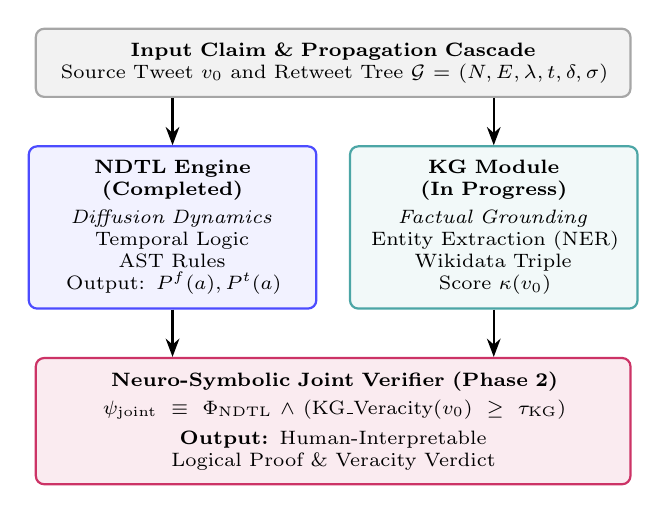
\begin{tikzpicture}[
    >=Stealth,
    node distance=0.7cm,
    every node/.style={font=\scriptsize, align=center},
    basebox/.style={draw, rounded corners=3pt, thick, fill=white, inner sep=5pt},
    inputbox/.style={basebox, draw=gray!70, fill=gray!10, text width=7.2cm},
    midbox/.style={basebox, text width=3.3cm, minimum height=1.6cm},
    jointbox/.style={basebox, draw=purple!80, fill=purple!8, text width=7.2cm}
]

    % Top Node
    \node[inputbox] (input) {\textbf{Input Claim \& Propagation Cascade}\\Source Tweet $v_0$ and Retweet Tree $\mathcal{G} = (N, E, \lambda, t, \delta, \sigma)$};

    % Middle Nodes (Side-by-side)
    \node[midbox, draw=blue!70, fill=blue!5, below left=0.6cm and 0.2cm of input.south] (ndtl) {
        \textbf{NDTL Engine (Completed)}\\[2pt]
        \textit{Diffusion Dynamics}\\
        Temporal Logic AST Rules\\
        Output: $P^f(a), P^t(a)$
    };

    \node[midbox, draw=teal!70, fill=teal!5, below right=0.6cm and 0.2cm of input.south] (kg) {
        \textbf{KG Module (In Progress)}\\[2pt]
        \textit{Factual Grounding}\\
        Entity Extraction (NER)\\
        Wikidata Triple Score $\kappa(v_0)$
    };

    % Bottom Node cleanly placed below mid nodes
    \node[jointbox, below=0.6cm of $(ndtl.south)!0.5!(kg.south)$] (joint) {
        \textbf{Neuro-Symbolic Joint Verifier (Phase 2)}\\[2pt]
        $\psi_{\text{joint}} \equiv \Phi_{\text{NDTL}} \land (\text{KG\_Veracity}(v_0) \ge \tau_{\text{KG}})$\\[3pt]
        \textbf{Output:} Human-Interpretable Logical Proof \& Veracity Verdict
    };

    % Clean Straight Downward Arrows (No Crossing Text)
    \draw[->, thick] (input.south -| ndtl.north) -- (ndtl.north);
    \draw[->, thick] (input.south -| kg.north) -- (kg.north);
    \draw[->, thick] (ndtl.south) -- (ndtl.south |- joint.north);
    \draw[->, thick] (kg.south) -- (kg.south |- joint.north);

\end{tikzpicture}%
}
\caption{System architecture coupling the completed NDTL diffusion engine with the ongoing Knowledge Graph factual verification module.}
\label{fig:kg_architecture}
\end{figure}

While NDTL achieves strong explainability by formalizing \textit{how} information diffuses, it remains agnostic to \textit{what} factual entities are asserted in the original claim. A cascade originating from a genuine emergency may exhibit viral burstiness mimicking disinformation, yielding false positives.

To resolve this limitation, we are actively constructing a \textbf{Knowledge Graph (KG) Grounding Module} to operate in tandem with the verified NDTL engine, as depicted in Figure~\ref{fig:kg_architecture}:
\begin{enumerate}
    \item \textbf{Entity Extraction \& Relation Linking:} Natural entity recognition (NER) extracts named entities and subject-predicate-object triples $\mathcal{T} = \{(h, r, t)\}$ from the preserved root tweet text in \texttt{filtered\_source\_tweets.txt}.
    \item \textbf{Triple Verification over Wikidata/DBpedia:} Candidate assertions are verified via SPARQL endpoints and projected into a pretrained TransE knowledge graph embedding space to compute semantic factual veracity:
    \begin{equation}
    \kappa(v_0) = \frac{1}{|\mathcal{T}|} \sum_{(h,r,t) \in \mathcal{T}} \sigma(f(h, r, t)).
    \end{equation}
    \item \textbf{Extended Temporal-Factual Logic (NDTL-KG):} Atomic factual predicates are integrated into NDTL syntax to produce a joint verification rule:
    \begin{equation}
    \psi ::= \varphi_{\text{NDTL}} \land (\text{KG\_Veracity}(v_0) \ge \tau_{\text{KG}}).
    \end{equation}
\end{enumerate}
The KG pipeline is currently under active construction and will be integrated into the final evaluation framework.

% =========================================================================
\section{Conclusion}
% =========================================================================

This project successfully reproduced the computational framework of News-Diffusion Temporal Logic (NDTL) for explainable fake news detection. All algorithmic components—including formal grammar parsing, AST model checking, threshold discovery, and decision rules—were implemented and verified. Furthermore, we diagnosed and eliminated an exponential path-traversal bottleneck in the reference implementation, achieving a 9.2\,ms execution speed. Experimental evaluations on synthetic networks and Twitter15/Twitter16 datasets confirmed that temporal logic effectively captures structural diffusion signals without black-box opacity. Active ongoing work focuses on completing and interfacing the Knowledge Graph (KG) grounding module to deliver a comprehensive neuro-symbolic misinformation verification platform.

% =========================================================================
% References
% =========================================================================
\begin{thebibliography}{99}

\bibitem{fionda2025logic}
V.~Fionda, ``Logic-based analysis of fake news diffusion on social media,'' \textit{Social Network Analysis and Mining}, vol.~15, no.~1, p.~59, 2025.

\bibitem{vosoughi2018spread}
S.~Vosoughi, D.~Roy, and S.~Aral, ``The spread of true and false news online,'' \textit{Science}, vol.~359, no.~6380, pp.~1146--1151, 2018.

\bibitem{castillo2011information}
C.~Castillo, M.~Mendoza, and B.~Poblete, ``Information credibility on twitter,'' in \textit{Proceedings of the 20th International Conference on World Wide Web (WWW)}, pp.~675--684, 2011.

\bibitem{ma2016detecting}
J.~Ma, W.~Gao, P.~Mitra, S.~Kwon, B.~J.~Jansen, K.-F.~Wong, and M.~Cha, ``Detecting rumors from microblogs with recurrent neural networks,'' in \textit{Proceedings of the 25th International Joint Conference on Artificial Intelligence (IJCAI)}, pp.~3818--3824, 2016.

\bibitem{ma2017detect}
J.~Ma, W.~Gao, and K.-F.~Wong, ``Detect rumors in microblog posts using propagation structure via kernel learning,'' in \textit{Proceedings of the 55th Annual Meeting of the Association for Computational Linguistics (Volume 1: Long Papers)}, pp.~708--717, 2017.

\bibitem{ciampaglia2015computational}
G.~L.~Ciampaglia, P.~Shiralkar, L.~M.~Rocha, J.~Bollen, F.~Menczer, and A.~Flammini, ``Computational fact checking from knowledge networks,'' \textit{PLOS ONE}, vol.~10, no.~6, p.~e0128193, 2015.

\bibitem{bian2020rumor}
T.~Bian, X.~Xiao, T.~Xu, P.~Zhao, W.~Huang, Y.~Rong, and J.~Huang, ``Rumor detection on social media with bi-directional graph convolutional networks,'' in \textit{Proceedings of the AAAI Conference on Artificial Intelligence}, vol.~34, pp.~549--556, 2020.

\end{thebibliography}

\end{document}



this is the code of the first phase evaluation of project thesis
this is looking very nice and verythingn is good said sir
now i need to add our knowledge graph part and finish the thesis ...need final thesis 
give me complete accurate code..just add KG and the needed for it to finish 
</USER_REQUEST>
<ADDITIONAL_METADATA>
The current local time is: 2026-09-24T20:04:07+05:30.
</ADDITIONAL_METADATA>